Diffusion models have emerged as a powerful class of generative models, enabling the generation of high-quality, diverse samples across various domains, including images, text, and audio. To direct the generation process towards desired outcomes, various guiderail mechanisms have been developed, including explicit conditioning, classifier guidance, and classifier-free guidance. These mechanisms constrain the generative process, ensuring that the output adheres to specific criteria or characteristics, thereby enhancing the model's utility for practical applications.

\subsection{Explicit Conditioning}
Explicit conditioning involves providing the diffusion model with additional context or information, guiding the generation process towards a specific outcome. This can be in the form of textual descriptions, labels, or any form of metadata that describes the desired output characteristics. For instance, in image generation, a text description can serve as a condition to generate images that match the described content. The effectiveness of explicit conditioning lies in its ability to leverage the conditional distribution learned by the model to produce outputs that closely align with the provided context or information.

\subsection{Classifier Guidance}
Classifier guidance integrates a separate classifier model to steer the generation process of the diffusion model. The classifier is trained to distinguish between desirable and undesirable outputs based on predefined criteria. During generation, the gradient signals from the classifier are used to adjust the diffusion process, pushing the generated samples towards the characteristics identified as desirable. This method allows for fine-grained control over the generation process, enabling the production of outputs that meet specific quality or content standards.

\subsection{Classifier-Free Guidance}
Classifier-free guidance is a technique that eliminates the need for a separate classifier model. Instead, it leverages the inherent capability of the diffusion model to differentiate between various outcomes. This is achieved by intermittently conditioning the model on a null input (i.e., providing no specific guidance) and comparing the output against those generated with explicit conditioning. The difference in outputs guides the adjustment of the generation process, encouraging the model to produce samples that are more closely aligned with the desired conditions, even in the absence of a dedicated classifier. This approach simplifies the generation process, reducing the computational overhead and complexity associated with maintaining a separate classifier model. \cite*{CFG}

\subsection{Some other methods}
Each of these guidance mechanisms serves to constrain and direct the generation process of diffusion models, enabling the creation of outputs that meet specific criteria or exhibit desired characteristics. The choice of mechanism depends on the specific requirements of the application, including the level of control needed, the availability of conditional information, and computational constraints.


The ability to steer image diffusion models enhances personalization, customization, and task-specific image generation. Direct manipulation of the image diffusion process enables adjustments in color variations \cite{sdedit2021} and facilitates inpainting tasks \cite{blended2022}. Text-guided controls extend these capabilities through prompt modification, CLIP feature manipulation, and cross-attention adjustments \cite{makeascene2022, spatext2022, gligen2023, textualinversion2022, dreambooth2022, promptedit2022}. Techniques like encoding segmentation masks into tokens for image generation control in MakeAScene \cite{makeascene2022}, or mapping these masks into localized token embeddings in SpaText \cite{spatext2022}, showcase the diversity of approaches. GLIGEN \cite{gligen2023} introduces parameter adjustments in attention layers for more grounded generation processes. Personalization is further achieved through methods like Textual Inversion \cite{textualinversion2022} and DreamBooth \cite{dreambooth}, which fine-tune diffusion models using a collection of user-provided example images. Prompt-based editing methods \cite{promptedit2022} offer practical solutions for image manipulation. Furthermore, optimization techniques that align the diffusion process with sketches have been proposed \cite{sketchdiffusion2022}, alongside studies like MultiDiffusion \cite{multidiffusion2023}, which explore various control strategies over diffusion models.

\subsection{ControlNet}

\cite*{ControlNet} presents ControlNet, a novel neural network architecture designed to incorporate spatial conditioning controls into large pre-trained text-to-image diffusion models. ControlNet leverages the depth and robustness of the encoding layers from these pre-trained models, providing a powerful backbone for learning a variety of conditional controls. By employing "zero convolutions," which are convolution layers initialized with zeros, ControlNet ensures a seamless and noise-free integration of conditions into the diffusion process. This architecture allows for the manipulation of images using various conditions, such as edges, depth, segmentation, and human pose, with or without accompanying text prompts. The experiments demonstrate that ControlNet can effectively handle single or multiple conditions and is robust across different dataset sizes. It offers significant advancements in controlled image generation, potentially broadening the application scope of diffusion models in image editing, content creation, and beyond.








\definecolor{hidden-draw}{RGB}{161,165,193}
\definecolor{hidden-pink}{RGB}{244,243,250}
\begin{figure}[H]
    \centering
    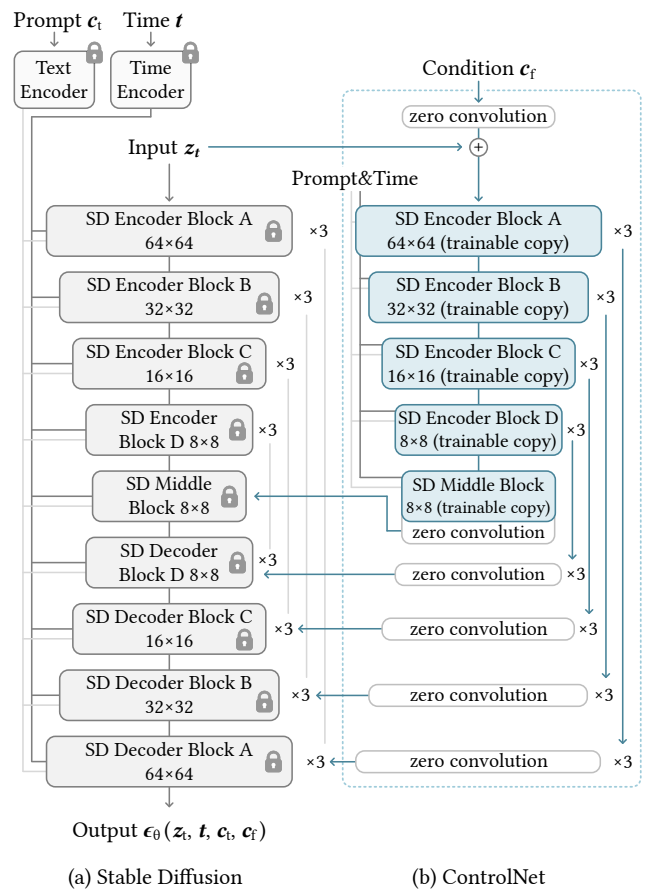
\includegraphics[width=0.60\textwidth]{images/controlnet.png} % Adjust the width as needed
    \caption{ControlNet: Guiding model through Canny, Depth Map, Pose Map, etc. \cite*{ControlNet}}
\end{figure}


\begin{figure}[H]
    \centering
    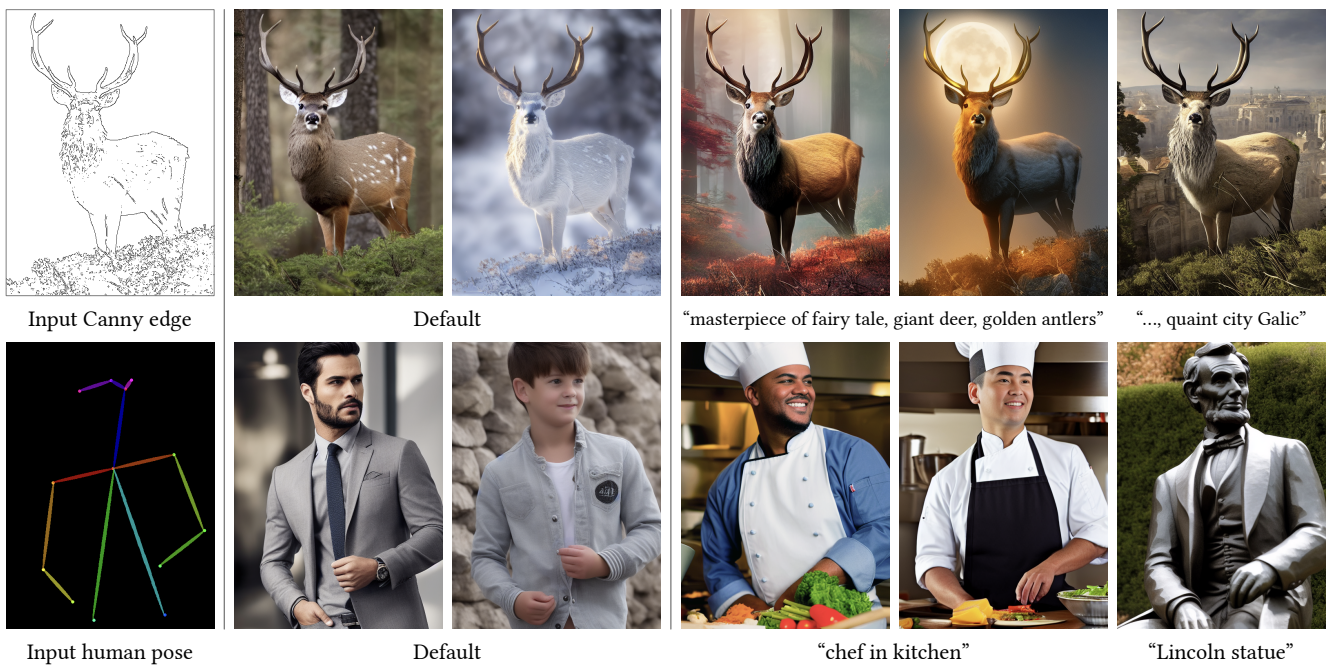
\includegraphics[width=1\textwidth]{images/controlnet_result.png}
    \caption{Controlling Stable Diffusion with learned conditions. ControlNet allows users to add conditions like Canny edges
    (top), human pose (bottom), etc., to control the image generation of large pretrained diffusion models. The default results use
    the prompt “a high-quality, detailed, and professional image”. Users can optionally give prompts like the “chef in kitchen”. \cite*{ControlNet}}
\end{figure}


% \tikzstyle{my-box}=[
%     rectangle,
%     draw=hidden-draw,
%     rounded corners,
%     text opacity=1,
%     minimum height=1.5em,
%     minimum width=5em,
%     inner sep=2pt,
%     align=center,
%     fill opacity=.5,
%     line width=0.8pt,
% ]
% \tikzstyle{leaf}=[my-box, minimum height=1.5em,
%     fill=hidden-pink!80, text=black, align=left,font=\tiny,
%     inner xsep=2pt,
%     inner ysep=4pt,
%     line width=0.8pt,
% ]


% \begin{figure*}[t!]
%     \centering
%     \resizebox{0.5\textwidth}{!}{
%         \begin{forest}
%             forked edges,
%             for tree={
%                 grow=east,
%                 reversed=true,
%                 anchor=base west,
%                 parent anchor=east,
%                 child anchor=west,
%                 base=left,
%                 font=\tiny,
%                 rectangle,
%                 draw=hidden-draw,
%                 rounded corners,
%                 align=left,
%                 minimum width=2em,
%                 edge+={darkgray, line width=1pt},
%                 s sep=3pt,
%                 inner xsep=2pt,
%                 inner ysep=3pt,
%                 line width=0.8pt,
%                 ver/.style={rotate=90, child anchor=north, parent anchor=south, anchor=center},
%             },
%             where level=1{text width=6em,font=\tiny,}{},
%             where level=2{text width=4.3em,font=\tiny,}{},
%             where level=3{text width=4.0em,font=\tiny,}{},
%             [
%                 Controllable Generation with Text-to-Image Diffusion Models, ver
%                 [
%                     Generation with \\ specific condition (\S \ref{sec:method})
%                     [
%                         Personalization \\ (\S~\ref{sec:personalization})
%                         [
%                            \textbf{(a) Subject-Driven:} Textual Inversion\cite{gal2022image} {,} Dreambooth\cite{ruiz2023dreambooth} {,} Re-Imagen\cite{chen2022re} {,} DreamArtist\cite{dong2022dreamartist} {,} \\Custom Diffusion\cite{kumari2023multi} {,} DVAR\cite{voronov2023loss} {,} E4T\cite{gal2023designing} {,} ELITE\cite{wei2023elite} {,} UMM-Diffusion\cite{ma2023unified} {,} XTI\cite{voynov2023p+} {,} SVDiff\cite{han2023svdiff} {,} \\ANOVA\cite{xiang2023closer} {,} SuTI\cite{chen2023subject} {,} Jia \emph{et al.}\cite{jia2023taming} {,} InstantBooth\cite{shi2023instantbooth} {,} COTI\cite{yang2023controllable} {,} Gradient-Free TI\cite{fei2023gradient} {,} Perfusion\cite{tewel2023key} {,} \\DisenBooth\cite{chen2023disenbooth} {,} BLIP-Diffusion\cite{li2023blip} {,} ProSpect\cite{zhang2023prospect} {,} Break-A-Scene\cite{avrahami2023break} {,} COMCAT\cite{xiao2023comcat} {,} OFT\cite{qiu2023controlling} {,} \\PACGen\cite{li2023generate} {,} Arar \etal\cite{arar2023domain} {,} Subject-Diffusion\cite{ma2023subject} {,} LyCORIS\cite{yeh2023navigating} {,} Kosmmos-G\cite{pan2023kosmos} {,} MCPL\cite{jin2023image} {,} \\He \emph{et al.}\cite{he2023data} {,} KC Loss\cite{roy2023diffnat} {,} MATTE\cite{agarwal2023image} {,} Lego\cite{motamed2023lego} {,} CatVersion\cite{zhao2023catversion} {,} CLiC\cite{safaee2023clic} {,} VideoAssembler\cite{zhao2023videoassembler} {,} \\ HiFi Tuner\cite{wang2023hifi} {,} VideoBooth\cite{jiang2023videobooth} {,} CAFE\cite{zhou2023customization} {,} DETEX\cite{cai2023decoupled} {,} DreamTuner\cite{hua2023dreamtuner} \\
% 							\textbf{(b) Person-Driven:} FastComposer\cite{xiao2023fastcomposer} {,} Giambi \emph{et al.}\cite{giambi2023conditioning} {,} Face0\cite{valevski2023face0} {,} DreamIdentity\cite{chen2023dreamidentity} {,}\\ HyperDreamBooth\cite{ruiz2023hyperdreambooth} {,} PhotoVerse\cite{chen2023photoverse} {,} MagiCapture\cite{hyung2023magicapture} {,} Face-diffuser\cite{wang2023high} {,} $\mathscr{W}_+ $ Adapter\cite{li2023stylegan} {,}\\ RetriBooru\cite{tang2023retrieving} {,} FaceStudio\cite{yan2023facestudio} {,} ViscoNet\cite{cheong2023visconet} {,} DemoCaricature\cite{chen2023democaricature} {,} PhotoMaker\cite{li2023photomaker} {,} Stellar\cite{achlioptas2023stellar} {,} \\PortraitBooth\cite{peng2023portraitbooth} \\
% 							\textbf{(c) Style-Driven:} StyleDrop\cite{sohn2023styledrop} {,} StyleCrafter\cite{liu2023stylecrafter} {,} ArtAdapter\cite{chen2023artadapter} {,} StyleAligned\cite{hertz2023style} {,} SAG\cite{pan2023towards} \\
% 							\textbf{(d) Interaction-Driven:} Reversion\cite{huang2023reversion} {,} AnimateDiff\cite{guo2023animatediff} {,} MotionDirector\cite{zhao2023motiondirector} {,} LAMP\cite{wu2023lamp} {,} SAVE\cite{song2023save} {,} \\Materzynska \emph{et al.}\cite{materzynska2023customizing} {,} DreaMoving\cite{feng2023dreamoving} {,} MotionCrafter\cite{zhang2023motioncrafter} {,} InteractDiffusion\cite{tian2023interactdiffusion} \\
% 							\textbf{(e) Image-Driven:} unCLIP\cite{ramesh2022hierarchical} {,} Versatile Diffusion\cite{xu2023versatile} {,} Prompt-Free Diffusion\cite{xu2023prompt} {,} Uni-ControlNet\cite{zhao2023uni} {,}\\ IP-Adapter\cite{ye2023ip} {,} ViscoNet\cite{cheong2023visconet} {,} Context Diffusion\cite{najdenkoska2023context} {,} FreeControl\cite{mo2023freecontrol} \\
% 							\textbf{(f) Distribution-Driven:} Cao \etal\cite{cao2023concept} {,} DreamDistribution\cite{nlong2023dreamdistribution} 
%                             , leaf, text width=26.5em
%                         ]                    
% 					]
%                     [
%                         Spatial Control\\ (\S~\ref{sec:spatial})
%                         [
%                            eDiff-I\cite{balaji2022ediffi} {,} LGP\cite{voynov2023sketch} {,} SpaText\cite{avrahami2023spatext} {,} GLIGEN\cite{li2023gligen} {,} Universal Guidance\cite{bansal2023universal} {,} LayoutDiffuse\cite{cheng2023layoutdiffuse} {,} \\MCM\cite{ham2023modulating} {,} FreeDoM\cite{yu2023freedom} {,} FLIS\cite{xue2023freestyle} {,} LayoutDiffusion\cite{zheng2023layoutdiffusion} {,} HumanSD\cite{ju2023humansd} {,} LCDG\cite{liu2023late} {,} \\Giambi \emph{et al.}\cite{giambi2023conditioning} {,} GeoDiffusion\cite{chen2023integrating} {,} Attention-Refocusing\cite{phung2023grounded} {,} ZestGuide\cite{couairon2023zero} {,} CAC\cite{he2023localized} {,} SSMG\cite{jia2023ssmg} {,} \\DenseDiffusion\cite{Kim2023DenseTG} {,} JointNet\cite{zhang2023jointnet} {,} HyperHuman\cite{liu2023hyperhuman} {,} Region\&Boundary\cite{f2007methods} {,} EOCNet\cite{wang2023enhancing} {,} \\MATTE\cite{agarwal2023image} {,} LoCo\cite{zhao2023loco} {,} AnyLens\cite{voynov2023anylens} {,} LRDiff\cite{qi2023layered} {,} Loose Control\cite{bhat2023loosecontrol} {,} DemoCaricature\cite{chen2023democaricature} {,} \\InteractDiffusion\cite{tian2023interactdiffusion} {,} FreeControl\cite{mo2023freecontrol} {,} Local Control\cite{zhao2023local} {,} SCEdit\cite{jiang2023scedit} {,} Ren \etal\cite{ren2023towards}
%                             , leaf, text width=26.5em
%                         ]                    
% 					]
% 					[
%                         Advanced \\Text-Conditioned \\ (\S~\ref{sec:advanced_text})
%                         [
%                            Structure Diffusion\cite{Feng2022TrainingFreeSD} {,} Attend-and-Excite\cite{chefer2023attend} {,} GlueGen\cite{qin2023gluegen} {,} Rich-text-to-image\cite{ge2023expressive} {,} SynGen\cite{rassin2023linguistic} {,} \\Tailored Visions\cite{chen2023tailored} {,} ParaDiffusion\cite{wu2023paragraph} {,} PEA-Diffusion\cite{ma2023pea}
%                             , leaf, text width=26.5em
%                         ]                    
% 					]
% 					[
%                         In-Context  (\S~\ref{sec:in-context})
%                         [
%                            Prompt Diffusion\cite{wang2023context} {,} iPromptDiff\cite{chen2023improving}
%                             , leaf, text width=10.5em
%                         ]                    
% 					]
% 					[
%                         Brain-Guided  (\S~\ref{sec:brain}), text width=5.4em
%                         [
%                            Mind-Vis\cite{chen2023seeing} {,} Takagi \etal\cite{takagi2023high} {,} Brain-Diffuser\cite{Ozcelik2023NaturalSR} {,} MindDiffuser\cite{lu2023minddiffuser} {,} Ni \etal\cite{ni2023natural} {,} \\DreamDiffusion\cite{bai2023dreamdiffusion} {,} BrainVis\cite{fu2023brainvis}
%                             , leaf, text width=22.5em
%                         ]                    
% 					]
% 					[
%                         Sound-Guided  (\S~\ref{sec:sound}), text width=5.5em
%                         [
%                            GlueGen\cite{qin2023gluegen} {,} CAVT-MAE\cite{yang2023align}
%                             , leaf, text width=8.5em
%                         ]                    
% 					]
% 					[
%                         Text Rendering (\S~\ref{sec:text_rendering}), text width=5.5em
%                         [
%                            Liu \etal\cite{liu2022character} {,} GlyphDraw\cite{ma2023glyphdraw} {,} TextDiffuser\cite{chen2023textdiffuser} {,} GlyphControl\cite{yang2023glyphcontrol} {,} AnyText\cite{tuo2023anytext} {,} \\TextDiffuser-2\cite{chen2023textdiffuser2} {,} UDiffText\cite{zhao2023udifftext} {,} Diff-Text\cite{zhang2023brush}
%                             , leaf, text width=24.8em
%                         ]                    
% 					]
% 				]
% 				[
% 					Generation with \\ multiple conditions (\S~\ref{sec:multi-conditon})
% 					[
%                         Joint Training  (\S~\ref{sec:multi_joint}), text width=5em
%                         [
%                            Composer\cite{huang2023composer} {,} SVDiff\cite{han2023svdiff} {,} FastComposer\cite{xiao2023fastcomposer} {,} Cocktail\cite{hu2023cocktail}
%                             , leaf, text width=16.5em
%                         ]                    
% 					]
% 					[
%                         Continual Learning (\S~\ref{sec:multi_continual}), text width=6.8em
%                         [
%                            C-LoRA\cite{smith2023continual} {,} L$^2$DM\cite{sun2023create} {,} STAMINA\cite{smith2023continual2}
%                             , leaf, text width=11.5em
%                         ]                    
% 					]
% 					[
%                         Weight Fusion  (\S~\ref{sec:multi_fusion}), text width=5.2em
%                         [
%                            Custom Diffusion\cite{kumari2023multi} {,} Cones\cite{liu2023cones} {,} Mix-of-Show\cite{gu2023mix} {,} ZipLoRA\cite{shah2023ziplora} {,} Orthogonal Adaptation\cite{po2023orthogonal}
%                             , leaf, text width=25.5em
%                         ]                    
% 					]
% 					[
%                         Attention-based Integration (\S~\ref{sec:multi_attention}), text width=8.5em
%                         [
%                            Mix-of-Show\cite{gu2023mix} {,} Cones2\cite{liu2023cones2}
%                             , leaf, text width=9.5em
%                         ]                    
% 					]
% 					[
%                         Guidance Composition (\S~\ref{sec:multi_guidance}), text width=7.5em
%                         [
%                            Decompose and Realign\cite{wang2023decompose} {,} Face-diffuser\cite{wang2023high} {,} Cao \etal\cite{cao2023concept}
%                             , leaf, text width=16.5em
%                         ]                    
% 					]
% 				]
% 				[
% 					Universal Controllable \\ Generation (\S~\ref{sec:universal})
% 					[
%                         Conditional Score Prediction (\S~\ref{sec:uni_cond}), text width=8.5em
%                         [
%                            DiffBlender\cite{kim2023diffblender} {,} Emu2\cite{sun2023generative1}
%                             , leaf, text width=8.5em
%                         ]                    
% 					]
% 					[
%                         	Condition-Guided Score Estimation (\S~\ref{sec:uni_guide}), text width=10.5em
%                         [
%                            Universal Guidance\cite{bansal2023universal} {,} FreeDoM\cite{yu2023freedom} {,} SAG\cite{pan2023towards}
%                             , leaf, text width=14.5em
%                         ]                    
% 					]
% 				]
%             ]
%         \end{forest}
%     }
%     \caption{\textbf{Taxonomy of Controllable Generation}. From the condition perspective, we categorize controllable generation approaches into three sub-tasks, including generation with specific conditions, generation with multiple conditions, and universal controllable generation.}
%     \label{fig:taxonomy}
% \end{figure*}
